
\chapterimage{arquitectos-tenerife.jpg}
\chapter{Despliegue}

\section{Introducción}
En Software durante el proceso de despliegue se verifica que el producto funcione correctamente, esto implica que se cumpla con todos los requerimientos tanto funcionales como no funcionales, que se habían planteado, se incluye varias pruebas las cuales están orientadas a garantizar el mantenimiento del Software, ya que, por ejemplo, entre más acoplado y menos abstracto sea más difícil será el mantenimiento de este. El despliegue también se refiere al proceso de prueba durante y después de la liberación del producto, tales como la intalación de este, la creación de manuales y documentos para el manejo del Software y la capacitación del personal que va a hacer uso del programa, en este punto se llevan a cabo las siguientes actividades: Liberación, instalación y activación, desinstalación, actualización, seguimiento de versiones y adaptación\cite{Ospina_2012}.
\newpage

\section{Diagrama de Sistemas}

Los diagramas de sistemas o paquetes son esquemas que ayudan a visualizar la forma de organización de una arquitectura. Además de ello permite visualizar la dependencia que hay en cada uno de los sistemas para así mejorar su estructura. Dentro de los diagramas de sistemas es posible encontrar dependencias lineales o cíclicas, el objetivo en la mayoría de casos es que la dependencia sea lineal, pues si la dependencia es cíclica significa que hay algo mal diseñado, y es allí donde el diseño por componentes hace su entrada para aliviar dicho problema. 
Para el caso particular del Sistema de Gestión de Monitorias se tiene el siguiente diagrama de sistemas:

\begin{figure}[H]
	\centering
	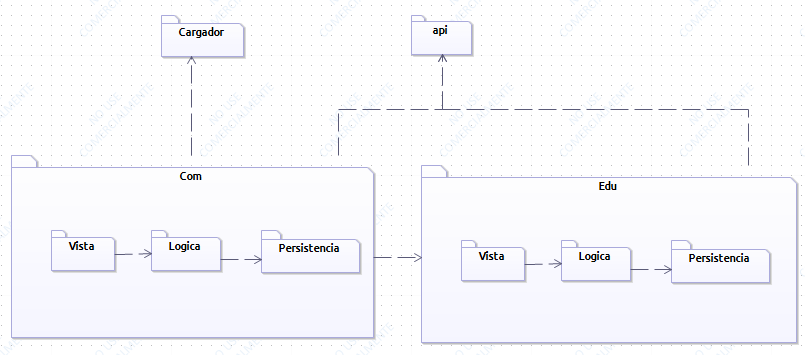
\includegraphics[width=1\linewidth]{dSistemas}
	\centering
	\caption{Diagrama de sistemas SGM}
	\label{fig:dSistemas}
\end{figure}

En el diagrama se aprecian dos grandes sistemas, Edu, el cuál abarca los subsistemas de Vista, Lógica y Persistencia correspondientes a cada componente y el cuál depende de un api. El otro sistema Com, también incluye los subsistemas de Edu, con la única diferencia de que este sistema es el aplicativo como tal, pues usa componentes, el cargador y un api.

\newpage

\section{Diagrama de Componentes}
\begin{figure}[H]
	\centering
	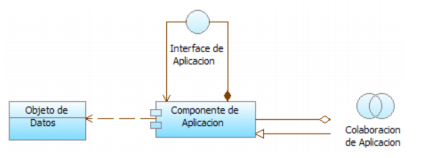
\includegraphics[width=0.7\linewidth]{componentes}
	\centering
	\caption{Estructura de un diagrama de componentes}
	\label{fig:componentes}
\end{figure}

El diagrama de componentes es similar a un diagrama de clases, pero da una visión más
general de la arquitectura del sistema. El diagrama de componentes muestra los componentes
del sistema, como un archivo de clases, un paquete, las bibliotecas compartidas, una base
de datos, etc., y cómo se relacionan entre sí. Los componentes individuales de un diagrama de
componentes se consideran en más detalle dentro de otros diagramas de UML, como los
diagramas de clases y los diagramas de casos de uso \cite{Kendall_2005}.

En el caso del sistema de Gestión de Monitoría, se planteó el diseño con 4 componentes básicos: El primero Clasificados, se encarga de gestionar la publicación y visualización de anuncios que los usuarios hagan en el sistema. El segundo componente, contactos gestiona las consultas de información de contacto de los participantes. El tercer componente, Monitorías, es el corazón del sistema, pues es allí donde se gestionan las horas y las certificaciones del aplicativo. Y por último el componente Perfil, gestiona toda la información del usuario, como su información personal y el número de horas que tienen los monitores.

\begin{figure}[H]
	\centering
	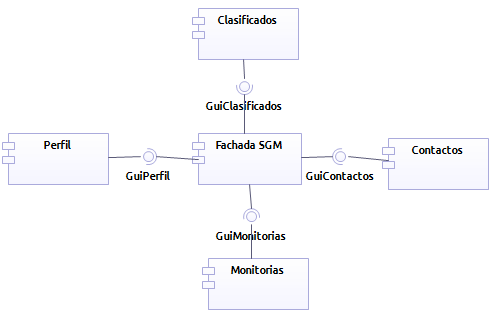
\includegraphics[width=0.7\linewidth]{dComponentes}
	\centering
	\caption{Diagrama de Componentes para el Sistema de Gestión de Monitorías}
	\label{fig:dcomponentes}
\end{figure}
\newpage


\section{Diagrama de Nodos}
El diagrama de nodos, como su nombre lo indica, representa un conjunto de nodos y la forma en la que se relacionan, este tipo de diagramas nos sirven para representar la forma en la que está estructurada la aplicación. Un nodo se define como un elemento físico que existe en tiempo de ejecución y representa un recurso computacional, que generalmente tiene alguna memoria y capacidad de procesamiento\cite{Nodos}.

\begin{figure}[H]
	\centering
	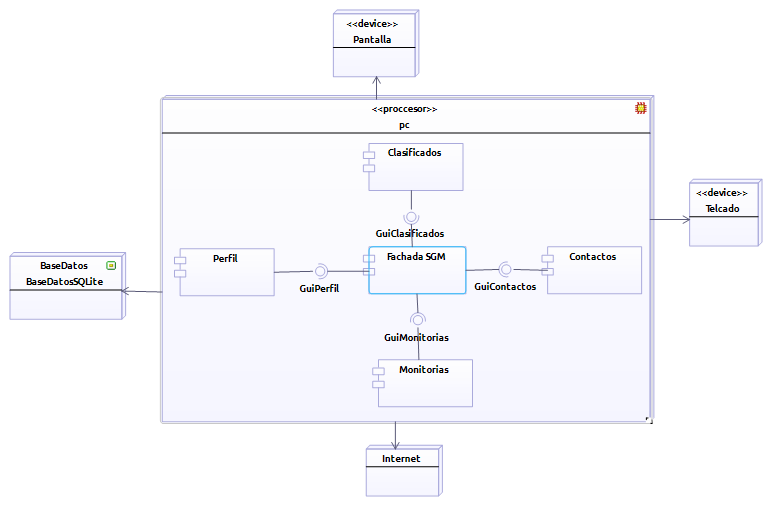
\includegraphics[width=0.9\linewidth]{dNodos}
	\centering
	\caption{Diagrama de nodos para el SGM.}
	\label{fig:dNodos}
\end{figure}
\newpage


\section{Métricas}

Una métrica consiste en un subconjunto de medidas que reúnen información sobre las características de un proyecto en particular. La esencia de las métricas es investigar las relaciones que hay entre las métricas de los procesos, las características del proyecto y la calidad del producto final, y, basado en los resultados ingeniar mejoras tanto en los procesos como en la calidad del producto \cite{Stehen_2003}.  

Existen diferentes tipos de métricas, tales como las siguientes:

\textbf{Métricas Contables} Dentro de estas métricas se encuentran los elementos contables del proyecto, tales como:
\begin{itemize}[itemsep=1mm,topsep=0pt,leftmargin=0.6in]
	\item\textbf{Libraries:} Número de librerías
	\item\textbf{Packages:} Número de paquetes
	\item\textbf{Units:} Número de clases de alto nivel
	\item\textbf{Units/Package:} Número promedio de clases de alto nivel por paquete
	\item\textbf{Classes/Class:} Número promedio de clases miembros por clase
	\item\textbf{Methods/Class:} Número promedio de métodos por clase.
	\item\textbf{Fields/Class:} Número promedio de campos por clase
	\item\textbf{ELOC:} Número estimado de líneas de código
	\item\textbf{ELOC/Unit:}  Número estimado de líneas de código por clase de alto nivel
\end{itemize}

\textbf{Métrica de Complejidad}
Estas métricas se encargan de medir cuantitativamente la complejidad lógica del software, estas ayudan a identificar que el código sea confiable y fácil de manejar. Dentro de estas métricas se pueden medir:
\begin{itemize}[itemsep=0mm,topsep=0pt,leftmargin=0.6in]
	\item\textbf{CC:} Mide la complejidad ciclomática. Toma una medida de mantenibilidad del código, la probabilidad de incluir fallos o el esfuerzo necesario para poder probar todos sus caminos\cite{ccmetric}.
	\item\textbf{Fat-libraries:} Fat para Dependencia de librerías
	\item\textbf{Unidades:} Número de clases de alto nivel
	\item\textbf{Fat-Packages:} Fat para dependencia de paquetes planos
	\item\textbf{Fat-Units:} Fat para clases de alto nivel
	\item\textbf{Tangled Libraries:} Porcentaje de librerías enredadas en las dependencias.
	\item\textbf{ACD Library:} Porcentaje promedio de dependencia de componentes entre librerías
	\item\textbf{ACD Packages:}Porcentaje promedio de dependencia de componentes entre paquetes
	\item\textbf{ACD Unit:}  Porcentaje promedio de dependencia de componentes entre unidades
\end{itemize}

\textbf{Métricas Robert C. Martin}
Estas métricas se encargan de concentrarse en las relaciones entre paquetes del proyecto. Dentro de estas se pueden encontrar:
\begin{itemize}[itemsep=0mm,topsep=0pt,leftmargin=0.6in]
	\item\textbf{D:} Distancia promedio, es un indicador de balance de los paquetes entre la abstracción y la inestabilidad.
	\item\textbf{|D|:} Valor absoluto de la distancia promedio
	\item\textbf{Ce:} Acoplamiento eferente, número de clases de un paquete que depende de clases de otro paquete externo
	\item\textbf{Ca:} Acoplamiento aferente, número de clases en otros paquetes que dependen del paquete analizado
	\item\textbf{I:} Grado de inestabilidad del paquete, es igual a Ce/(Ce+Ca)
	\item\textbf{A:} Grado de abstracción del paquete, es igual a 1-I
\end{itemize}

\textbf{Métricas Chidamber y Kemerer}
Este conjunto de métricas se utilizan para la medición de la calidad en el desarrollo de aplicaciones orientadas a objetos, principalmente estas métricas son orientadas a clase.
\begin{itemize}[itemsep=0mm,topsep=0pt,leftmargin=0.6in]
	\item\textbf{WMC:} Métodos ponderados por clase, calcula la suma de la complejidad ciclomática de los métodos de una clase.
	\item\textbf{DIT:} Profundidad en árbol de herencia, mide la distancia entre una clase a la raíz del árbol de herencia.
	\item\textbf{NOC:} Número de hijos inmediatos en el árbol de herencia, cuanto mayor sea este valor más reutilización habrá por herencia
	\item\textbf{CBO:} Acoplamiento entre clases, es el número de clases acopladas a una clase
	\item\textbf{RFC:} Respuesta para una clase, hace referencia al número de métodos que pueden ser ejecutados en respuesta a un mensaje recibido por un objeto de esa clase. 
	\item\textbf{LCOM:} Falta de cohesión entre métodos, mide la falta de cohesión de una determinada clase.
\end{itemize}

Para el caso de estudio del Sistema de Gestión de Monitorias, se usó el plugin STAN de Eclipse para encontrar las métricas asociadas al proyecto. Este plugin permite hallar las métricas mencionadas anteriormente y además de mostrar la polución del sistema, es decir la estabilidad del mismo. Y otro aspecto interesante que ofrece STAN es la posibilidad de visualizar la distancia (la relación entre abstracción e inestabilidad) para cada paquete.

\subsection{Proyecto SGM}

\textbf{Composición}
Aquí se pueden observar los paquetes por los que está compuesto el proyecto y sus dependencias.

\begin{figure}[H]
	\centering
	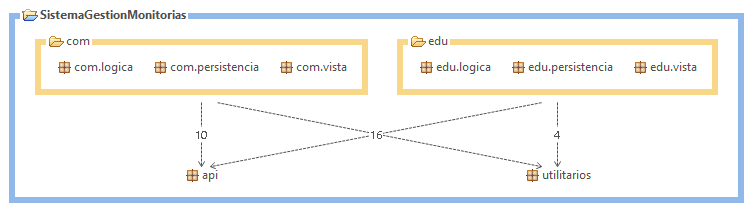
\includegraphics[width=1\linewidth]{mComposicion}
	\centering
	\caption{Composición del proyecto SGM}
	\label{fig:mComposicion}
\end{figure}
\textbf{Métricas Contables}
\begin{figure}[H]
	\centering
	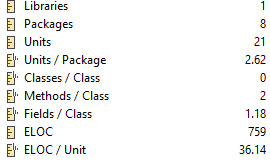
\includegraphics[width=0.6\linewidth]{mCount}
	\centering
	\caption{Métricas Contables para proyecto SGM.}
	\label{fig:mCount}
\end{figure}

\clearpage

\textbf{Métrica de Complejidad}
\begin{figure}[H]
	\centering
	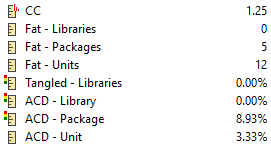
\includegraphics[width=0.6\linewidth]{mComplejidad}
	\centering
	\caption{Métricas de complejidad para proyecto SGM.}
	\label{fig:mComplejidad}
\end{figure}

\textbf{Métricas Robert C. Martin}
\begin{figure}[H]
	\centering
	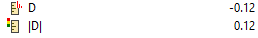
\includegraphics[width=0.6\linewidth]{mRobin}
	\centering
	\caption{Métricas Robert C. Martin para proyecto SGM.}
	\label{fig:mRobin}
\end{figure}
\textbf{Métricas Chidamber y Kemerer}
\begin{figure}[H]
	\centering
	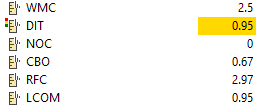
\includegraphics[width=0.6\linewidth]{mChidamber}
	\centering
	\caption{Métricas Chidamber y Kemerer para proyecto SGM.}
	\label{fig:mChidamber}
\end{figure}
\clearpage
\textbf{Polución}
\begin{figure}[H]
	\centering
	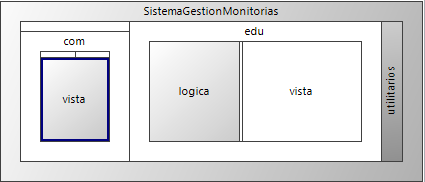
\includegraphics[width=0.8\linewidth]{mOverview}
	\centering
	\caption{Vistazo general a la polución del proyecto SGM.}
	\label{fig:mOverview}
\end{figure}
\begin{figure}[H]
	\centering
	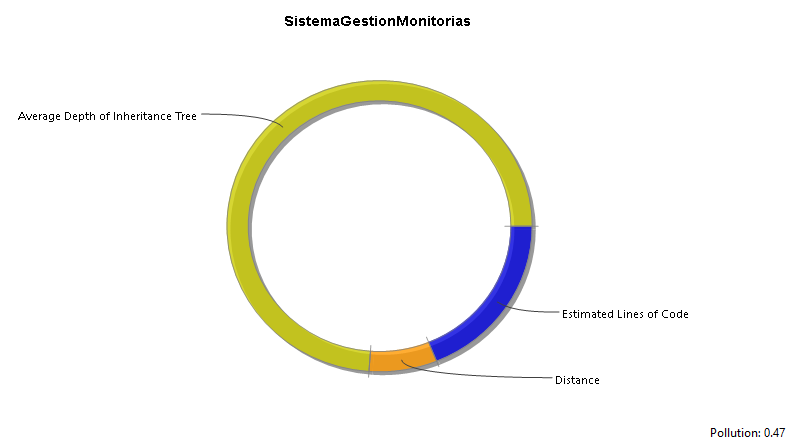
\includegraphics[width=0.8\linewidth]{mPolucion}
	\centering
	\caption{Polución para proyecto SGM.}
	\label{fig:mChidamber}
\end{figure}
\newpage
\subsection{Paquete API}

\textbf{Composición}
\begin{figure}[H]
	\centering
	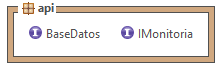
\includegraphics[width=0.4\linewidth]{mComposicionApi}
	\centering
	\caption{Composición del paquete api}
	\label{fig:mComposicionApi}
\end{figure}
\textbf{Acoplamiento}
\begin{figure}[H]
	\centering
	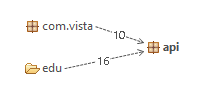
\includegraphics[width=0.4\linewidth]{mAcoplamientoApi}
	\centering
	\caption{Acoplamiento del paquete api}
	\label{fig:mAcoplamientoApi}
\end{figure}
\textbf{Métricas Contables}
\begin{figure}[H]
	\centering
	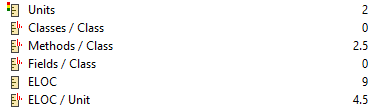
\includegraphics[width=0.6\linewidth]{mCountApi}
	\centering
	\caption{Métricas Contables del paquete api}
	\label{fig:mCountApi}
\end{figure}
\textbf{Métrica de Complejidad}
\begin{figure}[H]
	\centering
	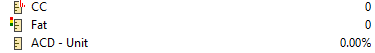
\includegraphics[width=0.6\linewidth]{mComplejidadApi}
	\centering
	\caption{Métricas de complejidad del paquete api.}
	\label{fig:mComplejidadApi}
\end{figure}

\textbf{Métricas Robert C. Martin}
\begin{figure}[H]
	\centering
	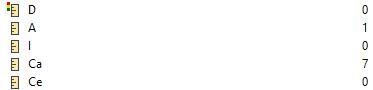
\includegraphics[width=0.6\linewidth]{mRobinApi}
	\centering
	\caption{Métricas Robert C. Martin para paquete api.}
	\label{fig:mRobinApi}
\end{figure}
\clearpage
\textbf{Métricas Chidamber y Kemerer}
\begin{figure}[H]
	\centering
	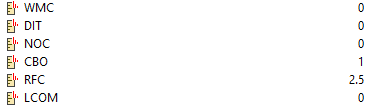
\includegraphics[width=0.6\linewidth]{mChidamberApi}
	\centering
	\caption{Métricas Chidamber y Kemerer del paquete api.}
	\label{fig:mChidamberApi}
\end{figure}
\textbf{Distancia}
\begin{figure}[H]
	\centering
	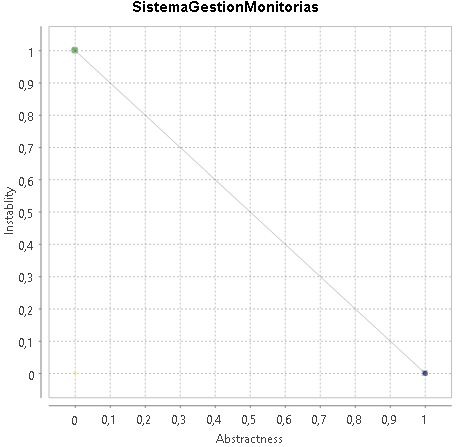
\includegraphics[width=0.8\linewidth]{mdistanciaApi}
	\centering
	\caption{Gráfico de distancia para el paquete api.}
	\label{fig:mdistanciaApi}
\end{figure}
\newpage
\subsection{Paquete utilitarios}

\textbf{Composición}
\begin{figure}[H]
	\centering
	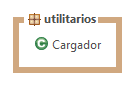
\includegraphics[width=0.2\linewidth]{mComposicionUtil}
	\centering
	\caption{Composición del paquete utilitarios.}
	\label{fig:mComposicionUtil}
\end{figure}
\textbf{Acoplamiento}
\begin{figure}[H]
	\centering
	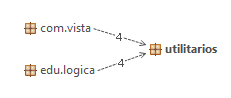
\includegraphics[width=0.4\linewidth]{mAcoplamientoUtil}
	\centering
	\caption{Acoplamiento del paquete utilitarios.}
	\label{fig:mAcoplamientoUtil}
\end{figure}
\textbf{Métricas Contables}
\begin{figure}[H]
	\centering
	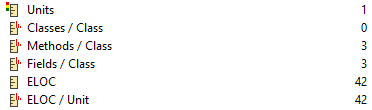
\includegraphics[width=0.6\linewidth]{mCountUtil}
	\centering
	\caption{Métricas Contables del paquete utilitarios}
	\label{fig:mCountApi}
\end{figure}
\textbf{Métrica de Complejidad}
\begin{figure}[H]
	\centering
	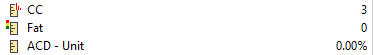
\includegraphics[width=0.6\linewidth]{mComplejidadUtil}
	\centering
	\caption{Métricas de complejidad del paquete utilitarios.}
	\label{fig:mComplejidadApi}
\end{figure}

\textbf{Métricas Robert C. Martin}
\begin{figure}[H]
	\centering
	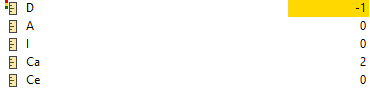
\includegraphics[width=0.6\linewidth]{mRobinUtil}
	\centering
	\caption{Métricas Robert C. Martin para paquete utilitarios.}
	\label{fig:mRobinUtil}
\end{figure}
\clearpage
\textbf{Métricas Chidamber y Kemerer}
\begin{figure}[H]
	\centering
	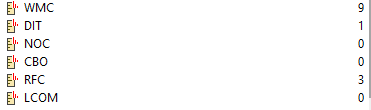
\includegraphics[width=0.6\linewidth]{mChidamberUtil}
	\centering
	\caption{Métricas Chidamber y Kemerer del paquete utilitarios.}
	\label{fig:mChidamberUtil}
\end{figure}
\textbf{Distancia}
\begin{figure}[H]
	\centering
	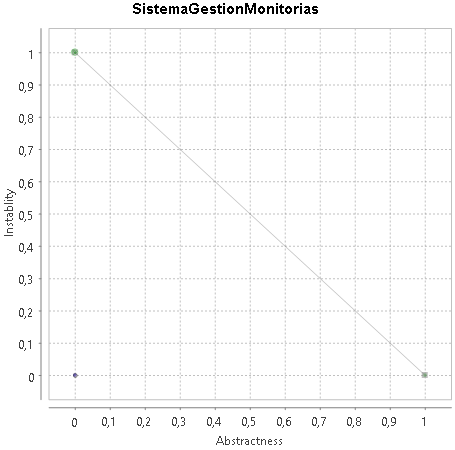
\includegraphics[width=0.8\linewidth]{mdistanciaUtil}
	\centering
	\caption{Gráfico de distancia para el paquete utilitarios.}
	\label{fig:mdistanciaUtil}
\end{figure}

\newpage
\subsection{Paquete Com}

\textbf{Composición}
\begin{figure}[H]
	\centering
	
\includegraphics[width=0.4\linewidth]{mComposicionCom}
	\centering
	\caption{Composición del paquete Com.}
	\label{fig:mComposicionCom}
\end{figure}
\textbf{Acoplamiento}
\begin{figure}[H]
	\centering
	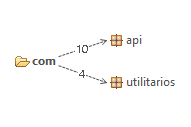
\includegraphics[width=0.4\linewidth]{mAcoplamientoCom}
	\centering
	\caption{Acoplamiento del paquete Com.}
	\label{fig:mAcoplamientoCom}
\end{figure}
\textbf{Métricas Contables}
\begin{figure}[H]
	\centering
	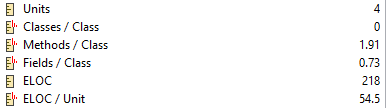
\includegraphics[width=0.6\linewidth]{mCountCom}
	\centering
	\caption{Métricas Contables del paquete Com.}
	\label{fig:mCountCom}
\end{figure}
\textbf{Métrica de Complejidad}
\begin{figure}[H]
	\centering
	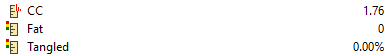
\includegraphics[width=0.6\linewidth]{mComplejidadCom}
	\centering
	\caption{Métricas de complejidad del paquete Com.}
	\label{fig:mComplejidadCom}
\end{figure}
\clearpage
\textbf{Distancia}
\begin{figure}[H]
	\centering
	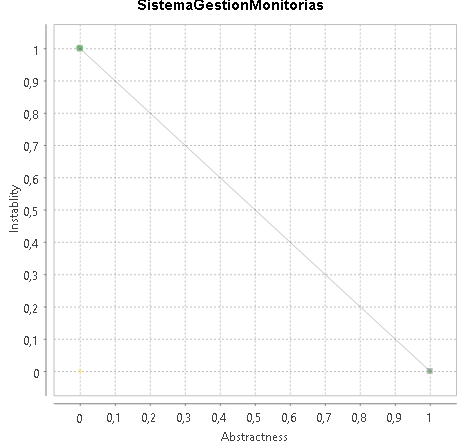
\includegraphics[width=0.8\linewidth]{mdistanciaCom}
	\centering
	\caption{Gráfico de distancia para el paquete Com.}
	\label{fig:mdistanciaCom}
\end{figure}

\newpage
\subsection{Paquete Edu}

\textbf{Composición}
\begin{figure}[H]
	\centering
	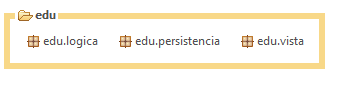
\includegraphics[width=0.4\linewidth]{mComposicionEdu}
	\centering
	\caption{Composición del paquete Edu.}
	\label{fig:mComposicionEdu}
\end{figure}
\textbf{Acoplamiento}
\begin{figure}[H]
	\centering
	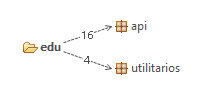
\includegraphics[width=0.4\linewidth]{mAcoplamientoEdu}
	\centering
	\caption{Acoplamiento del paquete Edu.}
	\label{fig:mAcoplamientoEdu}
\end{figure}
\textbf{Métricas Contables}
\begin{figure}[H]
	\centering
	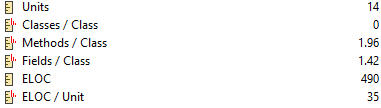
\includegraphics[width=0.6\linewidth]{mCountEdu}
	\centering
	\caption{Métricas Contables del paquete Edu.}
	\label{fig:mCountEdu}
\end{figure}
\textbf{Métrica de Complejidad}
\begin{figure}[H]
	\centering
	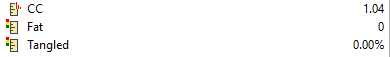
\includegraphics[width=0.6\linewidth]{mComplejidadEdu}
	\centering
	\caption{Métricas de complejidad del paquete Edu.}
	\label{fig:mComplejidadEdu}
\end{figure}
\clearpage
\textbf{Distancia}
\begin{figure}[H]
	\centering
	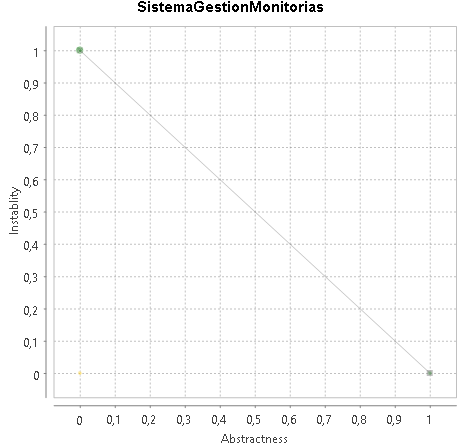
\includegraphics[width=0.8\linewidth]{mdistanciaEdu}
	\centering
	\caption{Gráfico de distancia para el paquete Edu.}
	\label{fig:mdistanciaEdu}
\end{figure}